\documentclass[12pt]{article}
\usepackage[T1]{fontenc} 
\usepackage[portuguese]{babel}
\usepackage{hyphenat}
% use se você precisar forçar a separação de sílabas em quebra de linha
\hyphenation{mate-mática recu-perar}
\usepackage{graphicx}
\graphicspath{images/}
\usepackage{csquotes}
\usepackage{subfiles}
\usepackage{amsmath}
\usepackage{csvsimple} 
\usepackage{geometry}
\geometry{
    a4paper,
    left=3cm,
    top = 3cm,
    right=2cm,
    bottom=2cm
}
\setlength{\parindent}{4em}
%\setlength{\parskip}{1em}
\renewcommand{\baselinestretch}{1.5}

\usepackage[dvipsnames]{xcolor}
\definecolor{alert}{RGB}{201, 58, 128}
\setlength {\marginparwidth }{2cm} 
\usepackage[colorinlistoftodos]{todonotes}
\usepackage{comment}
\usepackage{subcaption}
\DeclareUnicodeCharacter{0301}{*************************************}
\usepackage{enumitem}

\title{TÍTULO}
\author{autor}

\begin{document}

% CAPA
\thispagestyle{empty}

    
    \begin{flushright}
        \begin{huge}
            \textbf{RELATÓRIO}\\[3,5cm]
        \end{huge}

{\bf \LARGE  TÍTULO}

\bigskip
        
        (Orientando)\\
        Carlos da Silva dos Santos (Orientador)\\
        Universidade Federal do ABC\\[5,5cm]
    \end{flushright}
    
    \begin{center}
        Santo André,\\
        Junho de 2023
    \end{center}
    
    \newpage
\bigskip

\begin{center}
\noindent{\bf \Large Resumo}
\end{center}

\begin{quote}
[Contexto, visão geral do método, etc]
\end{quote}

\begin{center}
Santo André, junho de 2023
\end{center}

\newpage
\bigskip

\section{Introdução}
\label{sec:introducao}

Exemplo de citação: redes neurais~\cite{alexnet2012}.

Escrevendo em \emph{itálico} ou \textbf{negrito}.

Uma lista de itens
\begin{itemize}
 \item Um
 \item Dois
\end{itemize}

Agora com numeração:
\begin{enumerate}
    \item Primeiro
    \item Segundo
\end{enumerate}

Agora com sequência alfabética:
\begin{enumerate}[label=(\alph*)]
    \item Primeiro
    \item Segundo
\end{enumerate}

Exemplo de expressão matemática em meio ao texto: $x \in [0, 1]$, outro exemplo: $f(x) = \frac{1}{1+e^{-x}}$.

Exemplo de equação numerada e como referenciar: veja a equação~(\ref{eq:somatoria}).
\begin{equation}
    \label{eq:somatoria}
    p(x) = \sum_{x=1}^{10} \frac{1}{x^2}
\end{equation}

Para incluir uma equação sem numeração, use o símbolo * (veja no arquivo .tex):
\begin{equation*}
    \label{eq:somatoria2}
    p(x) = \sum_{x=1}^{10} \frac{1}{\exp({x})}
\end{equation*}


O restante do texto é organizado da seguinte maneira: em primeiro lugar, apresentamos os objetivos deste trabalho na Seção~\ref{sec:objetivo}. Em seguida... 

% Comentando parte do texto
\begin{comment}
Trecho de comentário, não é acrescido ao documento final
\end{comment}

\section{Objetivos}
\label{sec:objetivo}

\section{Revisão Bibliográfica}
\label{sec:revisao}

\subsection{Fundamentos de Aprendizado de Máquina}
\label{sec:aprendizado}

\subsection{Métricas de Classificação}
\label{sec:metricas}


\section{Materiais e Métodos} 
\label{sec:metodos}




\subsection{Conjuntos de dados}
\label{sec:dados}


\subsection{Recursos computacionais}
\label{sec:recursos}

Bibliotecas de software, infra-estrutura


\subsection{Resultados} 
\label{sec:resultados}


\begin{figure}[htb]
 \centering
 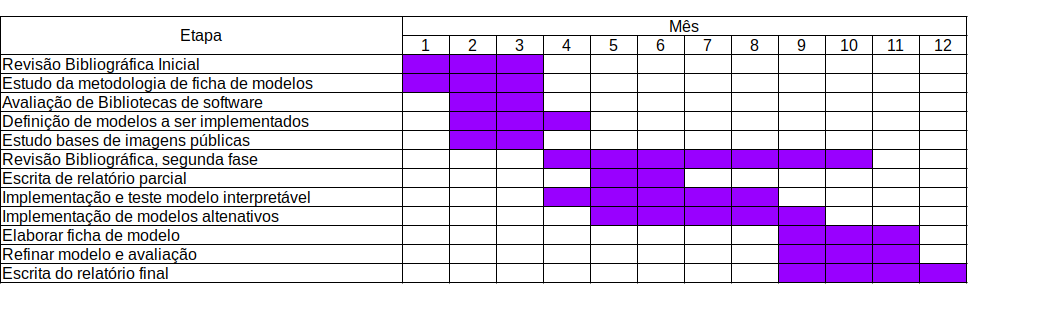
\includegraphics[width=1.0\textwidth]{images/crono2022}
 \caption{Cronograma de execução da proposta}
 \label{fig:crono}
\end{figure}


A Figura~\ref{fig:crono} apresenta o cronograma proposto...

\bibliographystyle{alpha}%{hapalike}
\bibliography{ref.bib}

\end{document}
